\begin{enumerate}
 \item
\begin{enumerate}
 \item Les coordonnées des points $M_1$ et $M_2$ sont respectivement
\begin{displaymath}
 M_1 : (d,b\sqrt{1-\frac{d^2}{a^2}}),\hspace{0.5cm} M_2 : (d,-b\sqrt{1-\frac{d^2}{a^2}})
\end{displaymath}
On en déduit les équations des droites en passant par des déterminants
\begin{multline*}
 M\in (A_1M_1)\Leftrightarrow
\begin{vmatrix}
 x(M) - a & d-a \\y(M) & b\sqrt{1-\frac{d^2}{a^2}}
\end{vmatrix}
=0 \\
\Leftrightarrow
b\sqrt{1-\frac{d^2}{a^2}}x(M)+(a-d)y(M) = ab\sqrt{1-\frac{d^2}{a^2}}\\
\end{multline*}
\begin{multline*}
M\in (A_2M_2)\Leftrightarrow
\begin{vmatrix}
 x(M) - a & d+a \\y(M) & -b\sqrt{1-\frac{d^2}{a^2}}
\end{vmatrix}
=0 \\
\Leftrightarrow
-b\sqrt{1-\frac{d^2}{a^2}}x(M) - (a+d)y(M) = ab\sqrt{1-\frac{d^2}{a^2}}
\end{multline*}
L'étude de l'intersection de ces deux droites revient à celle d'un système linéaires de deux équations à deux inconnues. On le traite avec des déterminants. Elles se coupent si et seulement si le déterminant noté $D$ du système est non nul. On trouve
\begin{displaymath}
 D = b\sqrt{1-\frac{d^2}{a^2}}
\begin{vmatrix}
  1 & a-d \\ -1 & -a-d
\end{vmatrix}
= -2db\sqrt{1-\frac{d^2}{a^2}}
\end{displaymath}
 Les deux droites se coupent si et seulement si $d\neq 0$.\newline
Les coordonnées du point d'intersection $I_d$ s'obtiennent avec les formules de Cramer. On calcule les déterminants
\begin{align*}
 &D_1= ab\sqrt{1-\frac{d^2}{a^2}} 
\begin{vmatrix}
 1 & a-d \\ 1 & -a-d
\end{vmatrix}
= -2a^2b\sqrt{1-\frac{d^2}{a^2}} \\
&D_2= b^2(1-\frac{d^2}{a^2}) 
\begin{vmatrix}
 1 & 1 \\ -1 & 1
\end{vmatrix}
= 2ab^2(1-\frac{d^2}{a^2})
\end{align*}
On en déduit les coordonnées du point d'intersection $I_d$:
\begin{displaymath}
 (\frac{a^2}{d}, -\frac{ab\sqrt{1-\frac{d^2}{a^2}}}{d})
\end{displaymath}

 \item Si $M$ est un point du plan pour lequel il existe un $d$ entre $-a$ et $a$ tel que $M=I_d$ alors $x(M)\neq 0$ et $d=\frac{a^2}{x(M)}$. En remplaçant dans la deuxième coordonnée, on obtient que l'équation demandée
\begin{multline*}
 \exists d\in [-a,a]\text{ tq } M=I_d \Leftrightarrow
\frac{y(M)}{b} = -\frac{x(M)}{a}\sqrt{1-\frac{a^2}{x(M)^2}}\\
\Leftrightarrow
\left\lbrace 
\begin{aligned}
 &\frac{y(M)^2}{b^2} = \frac{x(M)^2}{a^2}(1-\frac{a^2}{x(M)^2}) = \frac{x(M)^2}{a^2} -1 \\ &x(M)y(M)<0
\end{aligned}
\right. 
\end{multline*}
Il s'agit donc de la partie de l'hyperbole d'équation $\frac{x^2}{a^2} -\frac{y^2}{b^2}=1$ pour laquelle les abscisses et ordonnées ont des signes distincts.
\end{enumerate} 
\begin{figure}[h!t]
 \centering
 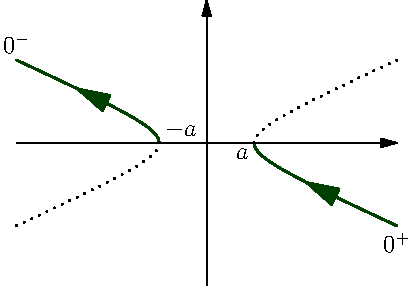
\includegraphics{./Cellipse1_1.pdf}
 \caption{Question 1.b. Les points d'intersection forment une partie d'hyperbole}
 \label{fig:Cellipse1_1}
\end{figure}

 \item
\begin{enumerate}
 \item Pour former l'équation de $\Gamma_d$ cercle de diamètre $M_1 M_2$, on écrit la nullité du produit scalaire.
\begin{displaymath}
 M\in \Gamma_d \Leftrightarrow (\overrightarrow{M_1M}/ \overrightarrow{M_2M}) = 0
\end{displaymath}
avec les coordonnées des vecteurs
\begin{displaymath}
 \overrightarrow{M_1M}:
\begin{pmatrix}
 x(M)-d \\ y(M)-b\sqrt{1-\frac{d^2}{a^2}}
\end{pmatrix}
\hspace{0.5cm}
 \overrightarrow{M_2M}:
\begin{pmatrix}
 x(M)-d \\ y(M)+b\sqrt{1-\frac{d^2}{a^2}}
\end{pmatrix}
\end{displaymath}
On en déduit l'équation de $\Gamma_d$.
\begin{displaymath}
 M\in \Gamma_d \Leftrightarrow
(x(M)-d)^2+ y(M)^2-b^2(1-\frac{d^2}{a^2})=0
\end{displaymath}

 \item Un point $M$ appartient à un $\Gamma_d$ si et seulement si il existe un $d\in ]-a,a[$ tel que
\begin{displaymath}
(x(M)-d)^2+ y(M)^2-b^2(1-\frac{d^2}{a^2})=0
\end{displaymath}
Formons l'équation du second degré d'inconnue $Z$
\begin{multline*}
(x(M)-Z)^2+ y(M)^2-b^2(1-\frac{Z^2}{a^2})=0 \\
\Leftrightarrow
(\frac{b^2}{a^2}+1)Z^2 -2x(M)Z+x(M)^2+y(M)^2-b^2=0 \hspace{0.5cm} (1)
\end{multline*}
Il s'agit de déterminer sous quelle condition cette équation admet une solution dans $]-a,a[$.
Son discriminant se met sous la forme
\begin{displaymath}
 -4\left(
\frac{b^2}{a^2}x(M)^2 + \frac{a^2+b^2}{a^2}y(M)^2 - (a^2+b^2)\frac{b^2}{a^2}
 \right) 
\end{displaymath}
Il est positif si et seulement si
\begin{displaymath}
 \frac{b^2}{a^2}x(M)^2 + \frac{a^2+b^2}{a^2}y(M)^2 \leq (a^2+b^2)\frac{b^2}{a^2}
\Leftrightarrow
\frac{x(M)^2}{a^2+b^2} + \frac{y(M)^2}{b^2}\leq 1
\end{displaymath}
On peut donc introduire le disque elliptique (fermé) dont le bord est l'ellipse (notée $\mathcal E$) d'équation
\begin{displaymath}
 \frac{x^2}{a^2+b^2} + \frac{y^2}{b^2} = 1
\end{displaymath}
Lorsque $M$ est à l'extérieur de ce disque, l'équation $(1)$ n'admet pas de solution réelle et aucun cercle $\Gamma_d$ ne passe par $M$.\newline
Lorsque $M$ est à l'intérieur du disque ouvert, l'équation admet bien au moins une solution réelle $d$. Mais $d$ est-il dans $]-a,a[$?\newline
Presque toujours! En effet, d'après la première forme de $(1)$:
\begin{displaymath}
 b^2(1-\frac{d^2}{a^2})=(x(M)-d)^2+y(M)^2\geq 0
\end{displaymath}
et l'inégalité est stricte sauf si $M$ est $A_1$ ou $A_2$ ce qui entraine que $d\in]-a,a[$. Par tous les points du disque elliptique ouvert (c'est à dire privé de son bord) sauf $A_1$ et $A_2$ passe un cercle $\Gamma_d$. Par tous les points du bord $\mathcal{ E}$ passe un seul cercle puisque l'équation du second degré admet une racine double. 
\end{enumerate}

 \item
\begin{enumerate}
 \item Le centre $\omega$ de $C_d$ est à l'intersection de l'axe des $x$ et de la normale en $M_1$ à l'ellipse. Pour former l'équation de la normale on commence par calculer les coordonnées d'un vecteur tangent en $M_1$ en utilisant une paramétrisation trigonométrique que l'in dérive
\begin{displaymath}
 f(\theta)= O + a\cos(\theta)\overrightarrow i + b\sin(\theta) \overrightarrow j,\hspace{0.5cm}
\overrightarrow f'(\theta) = -a\sin(\theta)\overrightarrow i + b\cos(\theta) \overrightarrow j
\end{displaymath}
avec $f(\theta)=M_1$ si et seulement si 
\begin{displaymath}
 a\cos(\theta) = d, \hspace{0.5cm}
b\sin (\theta) = b\sqrt{1-\frac{d^2}{a^2}}
\end{displaymath}
On en déduit les coordonnées d'un vecteur directeur de la normale
\begin{displaymath}
 \left( -a\sqrt{1-\frac{d^2}{a^2}}, \frac{bd}{a}\right) 
\end{displaymath}
puis l'équation de la normale
\begin{displaymath}
 -a\sqrt{1-\frac{d^2}{a^2}}(x-d)+\frac{bd}{a}(y-b\sqrt{1-\frac{d^2}{a^2}})=0
\end{displaymath}
Les coordonnées de $\omega$ satisfont à cette relation avec $y(\omega)=0$ d'où
\begin{displaymath}
 x(\omega) = (1-\frac{b^2}{a^2})d
\end{displaymath}

 \item Les foyers $F_1$ et $F_2$ ont pour coordonnées $(c,0)$ et $(-c,0)$ avec $c=\sqrt{a^2-b^2}$ donc $x(\omega)=\frac{c^2d}{a^2}$. On a alors
\begin{displaymath}
 (\overrightarrow{\omega F_1} / \overrightarrow{\omega F_2})=
(c-\frac{c^2d}{a^2})(-c-\frac{c^2d}{a^2}) = \frac{c^4d^2}{a^4} - c^2
\end{displaymath}
Le rayon $r$ du cercle $C_d$ est égal à $\omega M_1$:
\begin{displaymath}
 r^2=(d-x(\omega))^2+b^2(1-\frac{d^2}{a^2})
=\frac{b^4d^2}{a^4}+b^2-\frac{b^2d^2}{a^2}
=b^2-\frac{b^2c^2d^2}{a^4}
\end{displaymath}
On en déduit
\begin{displaymath}
 r^2 = -\frac{b^2}{c^2}(\overrightarrow{\omega F_1} / \overrightarrow{\omega F_2})
\end{displaymath}

\end{enumerate}

 \item
\begin{enumerate}
 \item Comme on connait le rayon et le centre de $C_d$, on peut former son équation 
\begin{multline*}
 M_0\in C_d \Leftrightarrow
(x_0-\frac{c^2d}{a^2})^2 +y_0^2 = b^2-\frac{b^2c^2d^2}{a^4}\\
\Leftrightarrow
d^2\frac{c^2}{a^4}(\underset{=a^2}{\underbrace{c^2+b^2}})-2\frac{c^2x_0}{a^2}d + x_0^2+y_0^2-b^2=0
\Leftrightarrow
\frac{c^2}{a^2}f_{M_0}(d)=0
\end{multline*}

 \item Lorsque par $M_0$ passe au moins un cercle $C_d$, l'équation du second degré $f_{M_0}(d)=0$ admet au moins une solution réelle donc son discriminant (réduit) $\Delta$ est positif ou nul. Exprimons $\Delta$
\begin{multline*}
 \Delta = x_0^2 -\frac{a^2}{c^2}(x_0^2+y_0^2-b^2)
=-\frac{b^2}{c^2}x_0^2-\frac{a^2}{c^2}y_0^2+\frac{a^2b^2}{c^2}\geq 0 \\
\Leftrightarrow
\frac{x_0^2}{a^2} + \frac{y_0^2}{b^2} \leq 1
\end{multline*}
 en divisant par $\frac{a^2b^2}{c^2}$. On en déduit que les points par lesquels passe au moins un cercle $C_d$ sont dans le disque elliptique de bord $E$.

\item Par définition de $f_{M_0}$:
\begin{multline*}
 f_{M_0}(a)=\frac{a^2}{c^2}\left(x_0^2+y_0^2-b^2+c^2-2\frac{x_0c^2}{a} \right)\\ 
= \frac{a^2}{c^2}\left((x_0-\frac{c^2}{a})^2 +y_0^2-b^2+c^2 -\frac{c^4}{a^2}\right) \\
= \frac{a^2}{c^2}\left((x_0-\frac{c^2}{a})^2 +y_0^2-\frac{b^4}{a^2}\right) 
\end{multline*}
On a donc
\begin{displaymath}
 u = \frac{c^2}{a},\hspace{0.5cm}v=\frac{b^4}{a^2}
\end{displaymath}

\item On montre comme plus haut que
\begin{displaymath}
 f_{M_0}(-a)=\frac{a^2}{c^2}\left((x_0+\frac{c^2}{a})^2 +y_0^2-\frac{b^4}{a^2}\right)  
\end{displaymath}
Si par un point $M_0$ passe deux cercles $C_{d_1}$ et $C_{d_2}$, alors $M_0$ est dans le disque elliptique (question b) et la fonction du second degré $f_{M_0}$ s'annule en $d_1$ et $d_2$ avec $-a<d_1<d_2<a$. Elle prend des valeurs négatives entre ses racines et positives à l'extérieur. On a donc $f_{M_0}(-a)$ et $f_{M_0}(a)$ strictement positifs ce qui signifie que $M_0$ est à l'extérieur des disques de rayon $r=\frac{b^2}{a}$ et de centres $\frac{c^2}{a}$ et $-\frac{c^2}{a}$. Comme 
\begin{displaymath}
 \frac{c^2}{a}=a-\frac{b^2}{a}=a-r
\end{displaymath}
Ces cercles sont tangents aux sommets de l'ellipse, notons les $\mathcal{D}_1$ et $\mathcal{D}_2$.\newline
Réciproquement, si $M_0$ est dans le disque elliptique et à l'extérieur de $\mathcal{D}_1$ et $\mathcal{D}_2$, alors $f_{M_0}(-a)$ et $f_{M_0}(a)$ sont strictement positifs. La fonction $f_{M_0}$ atteint sa valeur minimale négative en $x_0$ qui est strictement entre $-a$ et $a$. Elle s'annule donc en $d_1$ et $d_2$ avec $-a<d_1<x_0<d_2<a$ ce qui prouve que $C_{d_1}$ et $C_{d_2}$ passent par le point $M_0$.

\item On récapitule les résultats des questions précédentes.
\begin{itemize}
 \item Si $M_0$ est à l'extérieur du disque elliptique, aucun cercle $C_d$ ne passe par $M_0$.
 \item Si $M_0$ est à l'intérieur du disque elliptique et à l'extérieur de $\mathcal{D}_1$ et $\mathcal{D}_2$, deux cercles $C_d$ passent par $M_0$.
 \item Si $M_0$ est à l'intérieur du disque elliptique et à l'intérieur d'un seul des disques, un seul cercle passe par $M_0$. En effet, si par exemple $M_0$ est à l'intérieur du disque de centre négatif et à l'extérieur de l'autre alors $f_{M_0}(-a)<0$, $f_{M_0}(x_0)<0,  f_{M_0}(a)>0$. La fonction $f_{M_0}$ admet alors deux racines $d_1$ et $d_2$ vérifiant $d_1 < -a < x_0 < d_1 < a$.
 \item Dans le cas où les deux disques se coupent, ce qui ne se produit que si 
\begin{displaymath}
 -a+2r>4-2r \Leftrightarrow a<2r \Leftrightarrow a^2 < 2b^2
\end{displaymath}
Il ne passe aucun cercle par $M_0$ lorsque le point se trouve à l'intérieur des deux disques (figure 5 de l'énoncé). 
\end{itemize}
\end{enumerate}

\item Soit $C_{d_1}$ un cercle et $\omega_1$ son centre, il vérifie $x(\omega_1)=\frac{c^2d_1}{a^2}$. Ce cercle passe par $M_0$ si et seulement si $f_{M_0}(d_1)=0$. La tangente en $M_0$ est parallèle à la droite $(A_1,A_2)$ si et seulement si $\overrightarrow{\omega_1 M_0}$ est colinéaire à $\overrightarrow j$ ce qui se traduit par 
\begin{displaymath}
 \frac{c^2d_1}{a^2} = x_0 \Leftrightarrow d_1 = \frac{a^2 x_0 }{c^2}
\end{displaymath}
 En remplaçant dans l'expression de $f_{M_0}$, après simplification par $\frac{a^2}{c^2}$ la condition devient
\begin{displaymath}
 f_{M_0}(d_1)=0 \Leftrightarrow \frac{a^2x_0^2}{c^2 }-x_0^2 +y_0^2-b^2=0
\Leftrightarrow \frac{x_0^2}{c^2} + \frac{y_0^2}{b^2} = 1
\end{displaymath}
ce qui est l'équation réduite d'une ellipse. Il est à noter que l'axe focal n'est pas forcément le même. La condition de basculement vertical de cet axe est $a^2 = 2b^2$.
\begin{figure}[h!t]
 \centering
 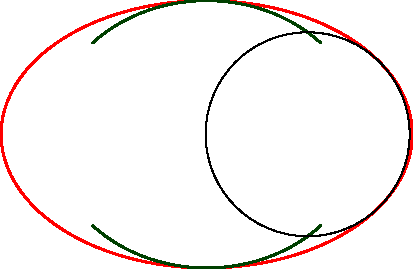
\includegraphics{./Cellipse1_2.pdf}
 % Cellipse1_2.pdf: 198x90 pixel, 72dpi, 6.99x3.17 cm, bb=0 0 198 90
 \caption{Tangente à $C_d$ parallele axe focal}
 \label{fig:Cellipse_1_2}
\end{figure}
Il faut aussi se limiter aux $x_0$ pour lesquels $|d_1|<a$. On obtient donc une partie de l'ellipse précédente.
\end{enumerate}

